\chapter{Introduction}
\section{Background}


Refactoring is a routine activity in software development: developers restructure code to improve readability, maintainability, and evolvability while keeping externally observable behaviour the same. Traditional definitions emphasise this preservation of behaviour and describe refactoring as a sequence of small, semantics-preserving transformations \cite{opdyke1992refactoring,fowler1999refactoring,fowler2018refactoring}, and subsequent surveys categorise these refactoring operations and the tools that support them \cite{mens2004survey}. In practice, refactoring is widely encouraged because poorly structured code becomes an obstacle when enhancing and maintaining code, and long-lived systems need continual adjustment (as argued in work building on Lehman’s laws and empirical studies of software maintenance). At the same time, refactoring can be costly: it consumes developer time, introduces risk, and is frequently intertwined with other work such as feature development and bug fixing rather than occurring as isolated “refactoring-only” tasks \cite{murphyhill2009howrefactor,kim2011apilevel}.

\section{Motivation}

Most research and tooling that evaluates refactoring focuses on \textit{outcomes} rather than the \textit{process}. A common approach is to measure refactoring success as a change in static quality indicators between a “before” and “after” state: reductions in code smells, improvements in cohesion/coupling, decreases in complexity, or related metrics to do with maintainability. Typical strands of work include metric-driven detection or prioritisation of candidate refactorings (e.g., using metric changes to separate refactoring-like edits from functional ones, or to choose between different refactoring options), as well as refactoring recommendation systems that rank alternatives by their impact on design metrics. More recent work expands the signals used for guidance by incorporating traceability alongside code metrics when ranking refactoring solutions, and exploring how product/process metrics relate to developers’ motivations to refactor (e.g., studies building on mined refactorings and repository history, and proposals that use LLMs to determine developers' motivations from commit artefacts). Alongside this, there is a substantial line of work that has improved the ability to \textit{detect} refactorings from code changes, notably by using AST-based differencing and structured matching to infer refactoring operations between revisions (e.g., RefactoringMiner and related approaches), which has enabled large-scale empirical studies of how often refactoring happens, what kinds occur, and in what contexts \cite{alikhanifard2025rminer,falleri2024gumtree}.

However, these perspectives evaluate refactoring as a mapping from an initial program state to a final program state, leaving the \textit{trajectory} between those states largely outside the picture. This matters because developers rarely refactor in a single atomic operation: they work through intermediate states, sometimes take detours, redo work, and often accept temporary degradation (e.g., in readability, modular structure, or test/build stability) before arriving at a final outcome. Two developers can arrive at the same end state via very different paths: one might take lots of disruptive steps, bounce between designs, or create avoidable churn, while another might get there via a steadier, more stable sequence. Existing endpoint-only evaluation cannot distinguish these different cases. Meanwhile, research on process realism suggests that refactoring is often ``flossed'' into ongoing development instead of being a separate dedicated task, which increases the chance of mixed-intent steps and noisy traces \cite{murphyhill2009howrefactor}. This makes the quality of the process (how a developer navigates intermediate states) potentially important for both developer productivity and the health of the codebase as it evolves.

Concurrent work has begun to analyse refactoring trajectories under a state/action/observation formalism, qualitatively classifying failure modes of language-model agents on multi-file refactoring tasks \cite{gautam2025refactorbench} and characterising recurring action patterns in software-engineering agent traces \cite{bouzenia2025trajectories}. A recent systematic literature review of LLM-based refactoring research likewise surveys evaluation methodologies and identifies open challenges in this area \cite{alomar2025slr}. As far as we are aware, however, no prior system both (i) scores a developer's refactoring trace against an explicit process-quality metric and (ii) produces counterfactual reference trajectories tied to measurable divergence points. The closest work either synthesises a path to reach an end state (without judging the developer's path) or recommends refactorings on an architectural target (without reference to an observed process). We instantiate the framing in a tool, evaluate it on a 45-session corpus of recorded refactoring sessions with hand-labelled ground truth, and report per-kind precision and recall alongside a sensitivity and ablation analysis of the underlying score formula.

\section{Research Objectives}

We investigate the following thesis question: \textbf{given a known start state and a known end state, can we evaluate the quality of the developer’s refactoring process, and identify points where a better process was available?} The core idea is to explicitly model refactoring as a \textit{process} over states, rather than judging it only by comparing endpoints. To do this, we adopt a state/action/trace framing: snapshots of the codebase are treated as \textit{states}, and developer edits---including IDE refactorings and manual transformations---are treated as \textit{actions} that produce a trace from the start state to the end state.

A core component will be a \textbf{process-quality metric} that scores traces according to criteria that will be defined and justified using existing research on code quality metrics, smell detection validity, and process-level signals. The metric is not assumed to be purely structural: it may incorporate multiple terms capturing endpoint improvement, intermediate-state degradation, churn/disruption, and “safety” proxies such as preserving build and test behaviour, reflecting the known limitations of relying on any one signal alone.

To go beyond scoring a single observed refactoring trace, we construct \emph{counterfactual} alternatives in the form of other \textbf{reference trajectories} between the same start and end states which have been optimised to achieve a higher score under a chosen process-quality metric. This provides a reasonable basis for comparison: analysis can identify \emph{divergence points} where the developer's trajectory deviates from a higher-scoring path, and quantify how much of the gap in resulting refactoring quality is due to each divergence. This extends previous work that synthesises or recommends refactoring sequences: ReSynth synthesises a path to reach a target end state from a developer's partial edits \cite{raychev2013resynth}, Refactoring Navigator suggests refactoring steps to guide a system toward a desired target at an architectural level \cite{lin2016navigator}, and search-based refactoring treats refactoring sequences as an optimisation problem under explicit quality functions \cite{harman2007pareto,mohan2019manyobjective}. While these systems show that refactoring sequences can be generated and optimised, they do not aim to assess the quality of a developer's chosen process under an explicit process-quality objective. In our work, counterfactual generation supports \emph{process evaluation}: it is used to construct a higher-scoring reference trajectory under the chosen metric and to explain key divergence points, rather than to automate the developer's work or to find any arbitrary sequence of steps that can be followed to reach the end state.

\section{Contributions}

Concretely, we make the following contributions:

\begin{itemize}
  \item A process-quality metric for refactoring trajectories, with each term grounded in cited prior work on code quality and developer process signals, and validated by a single-knob sensitivity sweep and a full power-set ablation analysis.
  \item A first-class divergence-point detector that classifies divergence into four kinds (\textsc{ordering}, \textsc{manual\_refactor}, \textsc{rework}, \textsc{hygiene}) and produces a counterfactual reference trajectory for each.
  \item A 45-session hand-recorded corpus on a purpose-built Java fixture, with multi-label ground-truth annotations, together with the experimental drivers (sensitivity, ablation, divergence) used to evaluate the detector against it.
  \item An empirical evaluation of the detector that establishes per-kind precision and recall, surfaces what the score formula measurably captures, and identifies which categories of process improvement the formula is structurally insensitive to.
\end{itemize}

\section{Approach and Scope}

Our approach targets refactoring as it actually occurs in real-world development, including sequences that involve both IDE-supported refactorings and manually performed edits. We initially focus on refactorings in a single language (Java) to allow the use of mature parsing infrastructure, established quality metrics, and state-of-the-art refactoring mining (e.g., RefactoringMiner). A refactoring process is represented as a sequence of steps between code snapshots. Steps may correspond to commits or developer-defined checkpoints, and this representation can be refined using higher granularity IDE data where available.

The final system comprises (i) an IDE plugin for capturing refactoring traces and presenting feedback, and (ii) an analysis component that scores the observed refactoring process and finds higher-scoring alternative trajectories between the same start and end states under a chosen process-quality metric. Rather than attempting all possible refactoring operators in a given state, or calculating globally optimal refactoring trajectories, the goal is to produce a plausible reference trajectory which scores higher on the chosen metric, and to explain the points at which the developer's trajectory diverged from it (e.g., where making a different earlier decision could have avoided churn, reduced temporary quality degradation, or preserved build/test stability).

\begin{figure}[H]
\centering
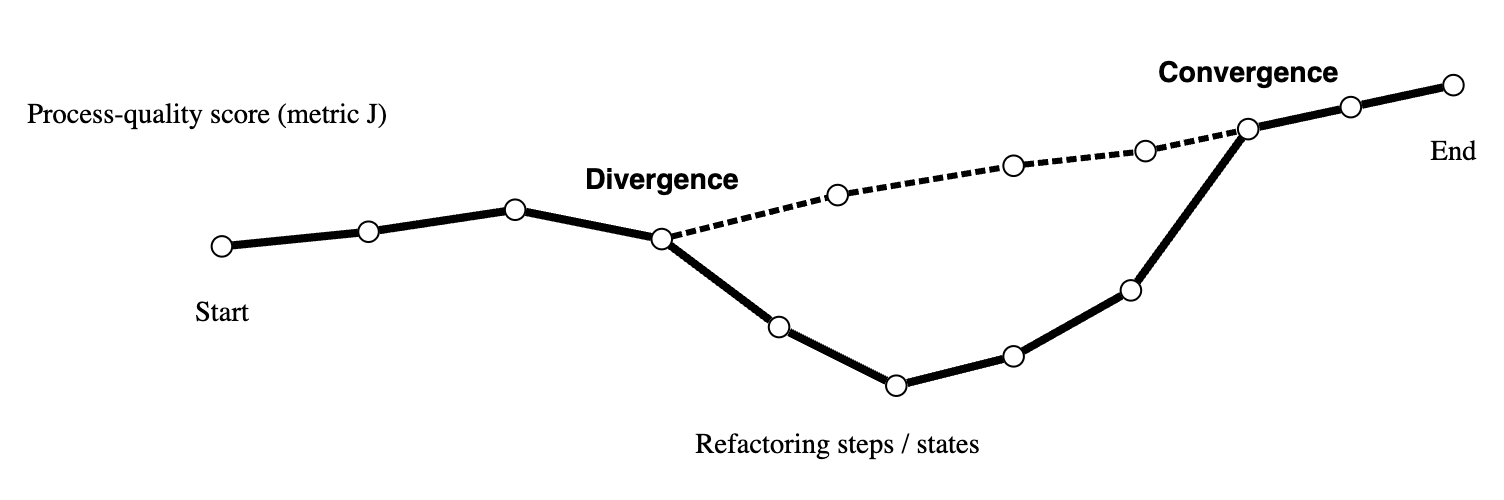
\includegraphics[width=0.8\textwidth]{introduction/divergence_diagram.png}
\caption{Illustration of refactoring trajectories scored by process-quality metric $J$. The solid line shows the developer's observed trajectory, and the dashed line shows a higher-scoring reference trajectory that diverges at an intermediate state and converges near the end.}
\label{fig:divergence}
\end{figure}

\section{Thesis Roadmap}
% TODO: update chapter cross-references to use \ref once the final chapter labels are in place.
The remainder of this thesis is structured as follows. Chapter~2 surveys related work in refactoring evaluation, mining, recommendation and synthesis, and positions our work against that literature. Chapter~3 defines the process-quality metric and the divergence-point detector. Chapter~4 describes the tool's architecture and implementation. Chapter~5 reports experimental results on the 45-session corpus and analyses threats to validity. Chapter~6 concludes and identifies directions for future work.
